\documentclass[a4paper,12pt]{article}
\usepackage{amsmath,amssymb,amsfonts,amsthm}
\usepackage{tikz}
\usepackage [utf8x] {inputenc}
\usepackage [T2A] {fontenc} 
\usepackage[russian]{babel}
\usepackage{cmap}
\usepackage{amsmath,amsfonts,amssymb,amsthm,mathtools} % AMS
\usepackage{graphicx}
\usepackage{wrapfig}
\usepackage{gensymb}
\usepackage{textcomp}
\usepackage{indentfirst}
\usepackage{floatrow}
\usepackage{multirow}
\usepackage{multicol} % Несколько колонок
\usepackage[version=3]{mhchem}
% вы сможете вставлять картинки командой \includegraphics[width=0.7\textwidth]{ИМЯ ФАЙЛА}
% получается подключать, как минимум, файлы .pdf, .jpg, .png.
\usepackage{mathtext} 				% русские буквы в фомулах
% Если вы хотите явно указать поля:
\usepackage[margin=1in]{geometry}
% Или если вы хотите задать поля менее явно (чем больше DIV, тем больше места под текст):
% \usepackage[DIV=10]{typearea}

\usepackage{fancyhdr}
\pagestyle{fancy}
\makeatletter % сделать "@" "буквой", а не "спецсимволом" - можно использовать "служебные" команды, содержащие @ в названии
\fancyhead[L]{\footnotesize Основы современной физики}%Это будет написано вверху страницы слева
\fancyhead[R]{\footnotesize ФЭФМ МФТИ}
\fancyfoot[R]{\thepage}%номер страницы —- внизу справа
\fancyfoot[C]{}%по центру внизу страницы пусто

\renewcommand{\maketitle}{%
	\noindent{\bfseries\scshape\large\@title\ \mdseries\upshape}\par
	\noindent {\large\itshape\@author}
	\vskip 2ex}
\makeatother
\def\dd#1#2{\frac{\partial#1}{\partial#2}}

\title{6.9.1 Закон Кюри-Вейсса и обменное взаимодействие в ферромагнетиках.}
\author{Богатова Екатерина} 
\date{\today}

\begin{document}
\maketitle
\textbf{Цель работы:} исследовать температурную зависимость магнитной восприимчивости ферромагнетика в парамагнитной области -- выше точки Кюри. По полученной в работе температуре Кюри оценить энергия обменного взаимодействия.

\section*{1. Теоретическая справка}
\subsection*{1.1 Феноменологическое описание ферромагнетиков: парамагнитная фаза и эффективное поле Вейсса}

Намагниченностью называется магнитный момент $І$ единицы объёма, который связан с внешним магнитным полем $H$ через магнитную восприимчивость $\varkappa$: $I = \varkappa H$

Рассмотрим восприимчивость парамагнитного вещества, в котором магнитный момент атома обусловлен только спином одного электрона. Тогда в магнитном поле у атома возникают два возможных уровня энергии: $E_{-}=-\mu B$ и $E_{+}=+\mu B$, причем в низкоэнергетичном состоянии $Е_-$ магнитный момент параллелен магнитному полю.

В соответствии с Больцмановским распределением отношение числа электронов $N_{+}$ с энергией $E_{+}$ к числу электронов $N_-$ с энергией $E_-$ равно

\begin{equation}\label{bolzman}
    \frac{N_{+}}{N_{-}}=\exp \left(-\frac{2 \mu B}{k_{\mathrm{B}} T}\right) \simeq 1-\frac{2 \mu B}{k_{\mathrm{B}} T}
\end{equation}

Намагниченность вещества определяется только разностью чисел электронов,
магнитные моменты которых ориентированы по полю или против поля, а поскольку мы рассматриваем проекцию магнитного момента на одну ось, то парамагнитная часть восприимчивости равна:

\begin{equation}\label{kappa-easy}
    \varkappa = \frac{I}{H} = N \frac{\mu^2}{k_B T} = N \frac{N g^{2} \mu_{\mathrm{B}}^{2} S(S+1)}{3 k_{\mathrm{B}} T}
\end{equation}

Для описания взаимодействия соседних электронов в ферромагнетике предположим, что в ферромагнетике имеется некоторое эффективное магнитное поле $H_{\text {эфф}}$. Величина обменного поля пропорциональна имеющейся намагниченности образца: $H_{\text{эфф}} = \lambda I$, где $\lambda$ -- некоторая константа. Тогда, учитывая поправку на дополнительное поле $H_{\text{эфф}}$, получим закон Кюри-Вейсса:

\begin{equation}\label{C-W}
    \varkappa=\frac{I}{H}=N \frac{g^{2} \mu_{\mathrm{B}}^{2} S(S+1)}{3 k_{\mathrm{B}}(T-\Theta)} \propto \frac{1}{T-\Theta}
\end{equation}

Где $\Theta=\frac{N \mu^{2} \lambda}{k_{\mathrm{B}}}=N \frac{g^{2} \mu_{\mathrm{B}}^{2} S(S+1)}{3 k_{\mathrm{B}}} \lambda$ -- параметр, имеющий размерность температуры.

Этот закон носит приближенный характер и не позволяет описать, что происходит в ферромагнитой области, но достаточно точно характеризует температурную зависимость магнитной восприимчивости в парамагнитной фазе. 

\subsection*{1.2 Связь эффективного поля Вейсса с обменным интегралом.}

Энергия обменного взаимодейтвия $U_\text{обм}$ атомов $i$ и $j$ представляет собой разность между средними значениями кулоновской энергии для параллельных и антипараллельных спинов $S_i$ и $S_j$, а $Ј$ -- коэффициент пропорциональности, называемый обменным интегралом, величина которого зависит от степени перекрытия распределённых зарядов атомов $i$ и $ј$.

\begin{equation}\label{energy}
    U_\text{обм} = -2 J S_i S_j
\end{equation}

Установим приближенно связь между обменным интегралом $Ј$ и константой Вейсса $\lambda$. Найдем энергию $U_\text{пер}$, требуемую для переворота данного спина в присутствии всех других спинов его ближайших соседей. С одной стороны, эта энергия вдвое больше обменной энергии системы с какой-то определенной ориентацией спина. С другой стороны, каждый магнитный атом испытывает действие эффективного поля, следовательно, воздействиевсех спинов на данный характеризуется средней намагниченностью $І=\mu/V$, и мы можем записать равенство

$$2\cdot2Jn S^2 = U_{\text{пep}}=2 \mu H_{\text{эфф}} =2 \mu \frac{\lambda \mu}{V}$$

Выразив константу $\lambda$ из температуры $\Theta$, мы получаем:

\begin{equation}\label{obm-int}
    J=\frac{3 k_{\text {B }} \Theta}{2 n S(S+1)}
\end{equation}

\section*{2. Экспериментальная установка и принцип измерений}

\begin{figure}[h!]
\begin{center}
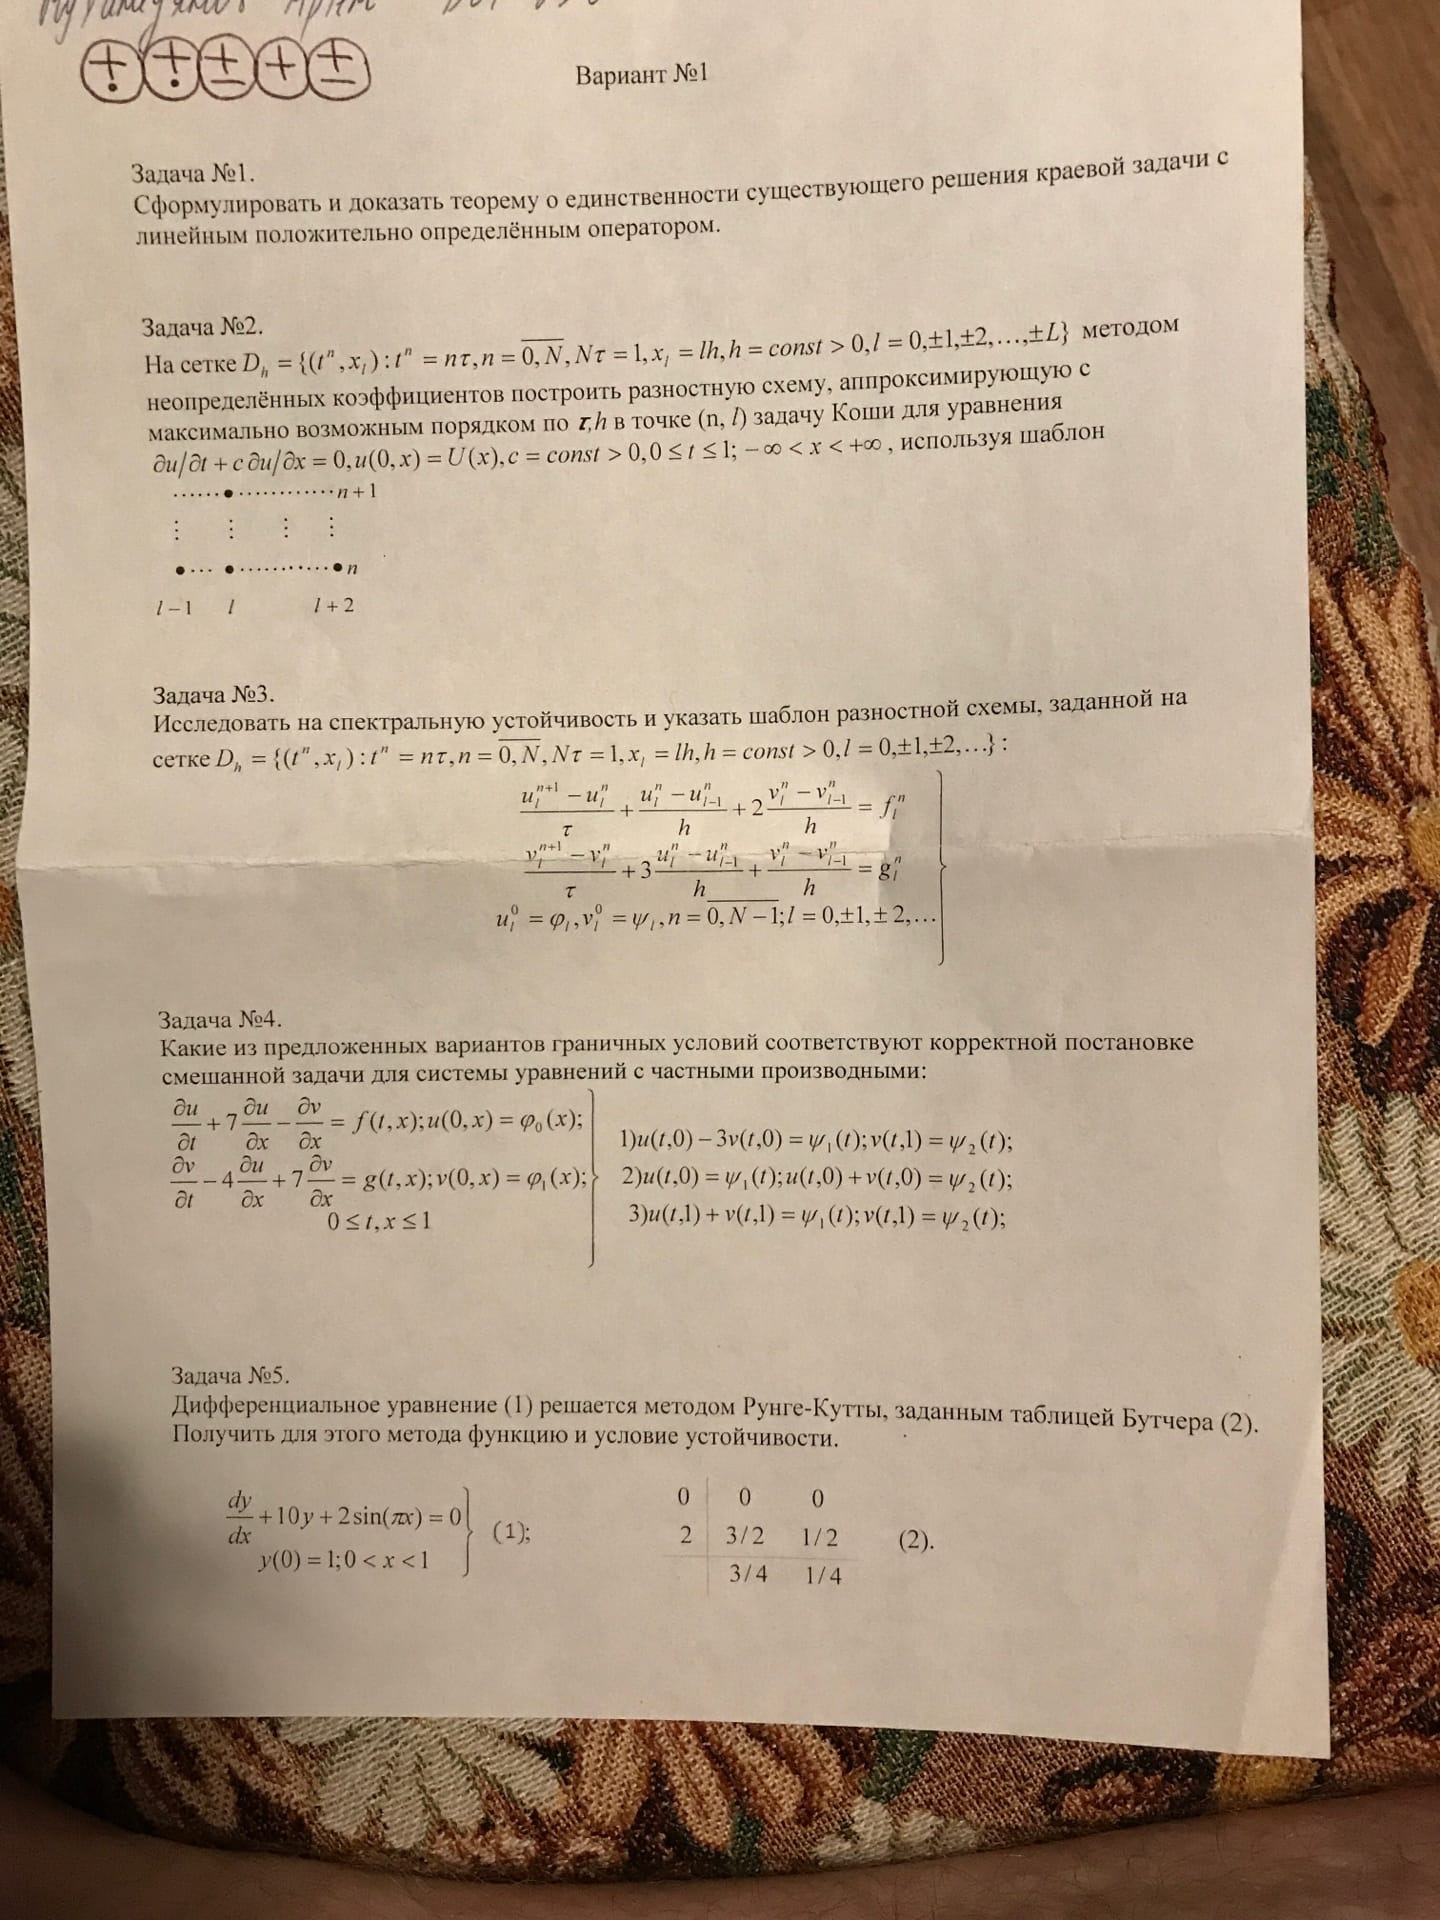
\includegraphics[scale=0.5]{1.jpg}
\caption{Схема экспериментальной установки}
\end{center}
\end{figure}

Экспериментальная установка для измерения восприимчивости магнетиков приведена на рис. 1.  Ферромагнитный образец 1 располагается внутри пустотелой катушки 2, которая является индуктивностью колебательного контура, входящего в состав LC-генератора. Частота колебаний генератора высвечивается на цифровом табло блока. Катушка самоиндукции помещена в термостат, представляющий собой массивный медный цилиндр 3, расположенный в пенопластовом корпусе 4. Образец помещен в тефлоновую капсулу. С помощью штока 5 капсулу можно перемещать вдоль оси катушки самоиндукции. Когда шток опущен, образец введен в катушку, а когда поднят -- образец из неё вынут.

Магнитная восприимчивость образца определяется по изменению самоиндукции, происходящему при его введении в катушку. Обозначая через $L$ индуктивность катушки с образцом и через $L_0$ её индуктивность в отсутствии образца, получим:

$$ \frac{L-L_{0}}{L_{0}}=\frac{\Delta L}{L_{0}}=\mu-1 = 4 \pi \varkappa$$

Учитывая, что частота $f$ колебательного LС-контура определяется выражением $\frac{1}{f}=2 \pi \sqrt{L C},$ получим:

\begin{equation}\label{dependency}
    \frac{1}{\varkappa} \propto \frac{f^{2}}{f_{0}^{2}-f^{2}}
\end{equation}  
	
\section*{3. Выполнение и обработка данных}
При выполнении работы образец сначала охлаждается ниже точки Кюри, а затем медленно нагревается. Исследуем зависимость частот $f$ и $f_0$ от температуры, постепенно нагревая образец. Измерения  проводим в интервале от $0~^\circ \text{C}$ до $50~^\circ \text{C}$ с шагом в примерно $3~^\circ \text{C}$, результаты представлены в Таблице 1.

\begin{table}[H]
\begin{tabular}{|l|l|l|l|l|l|l|l|l|}
\cline{1-4} \cline{6-9}
\multicolumn{1}{|c|}{U, мкВ} & \multicolumn{1}{c|}{T, $^\circ$С} & \multicolumn{1}{c|}{f$_0$, кГц} & \multicolumn{1}{c|}{f, кГц} &  & \multicolumn{1}{c|}{U, мкВ} & \multicolumn{1}{c|}{T, $^\circ$С} & \multicolumn{1}{c|}{f$_0$, кГц} & \multicolumn{1}{c|}{f, кГц} \\ \cline{1-4} \cline{6-9} 
-900                         & 1                         & 956,1                         & 909,2                       &  & 60                          & 24,5                      & 956                           & 947                         \\ \cline{1-4} \cline{6-9} 
-780                         & 4                         & 956,5                         & 909,3                       &  & 180                         & 27,4                      & 955,9                         & 950,4                       \\ \cline{1-4} \cline{6-9} 
-750                         & 4,7                       & 955,7                         & 909,6                       &  & 300                         & 30,3                      & 955,8                         & 951,9                       \\ \cline{1-4} \cline{6-9} 
-660                         & 6,9                       & 955,8                         & 909,8                       &  & 420                         & 33,2                      & 955,9                         & 952,7                       \\ \cline{1-4} \cline{6-9} 
-540                         & 9,8                       & 956                           & 909,9                       &  & 540                         & 36,2                      & 955,9                         & 953,1                       \\ \cline{1-4} \cline{6-9} 
-420                         & 12,8                      & 956,1                         & 910,6                       &  & 660                         & 39,1                      & 955,9                         & 953,4                       \\ \cline{1-4} \cline{6-9} 
-300                         & 15,7                      & 955,4                         & 913,4                       &  & 780                         & 42                        & 955,8                         & 953,9                       \\ \cline{1-4} \cline{6-9} 
-180                         & 18,6                      & 955,8                         & 923,4                       &  & 900                         & 45                        & 956                           & 954                         \\ \cline{1-4} \cline{6-9} 
-60                          & 21,5                      & 955,9                         & 939                         &  & 990                         & 47,1                      & 955,9                         & 954,1                       \\ \cline{1-4} \cline{6-9} 
\end{tabular} \caption{Результаты измерений.}
\end{table} 

Результаты измерения изорбразим на графике (Рис. 2) в координатах $\left( T, \frac{f^2}{f_0^2-f^2}\right)$.

\begin{figure}[H]
    \centering
    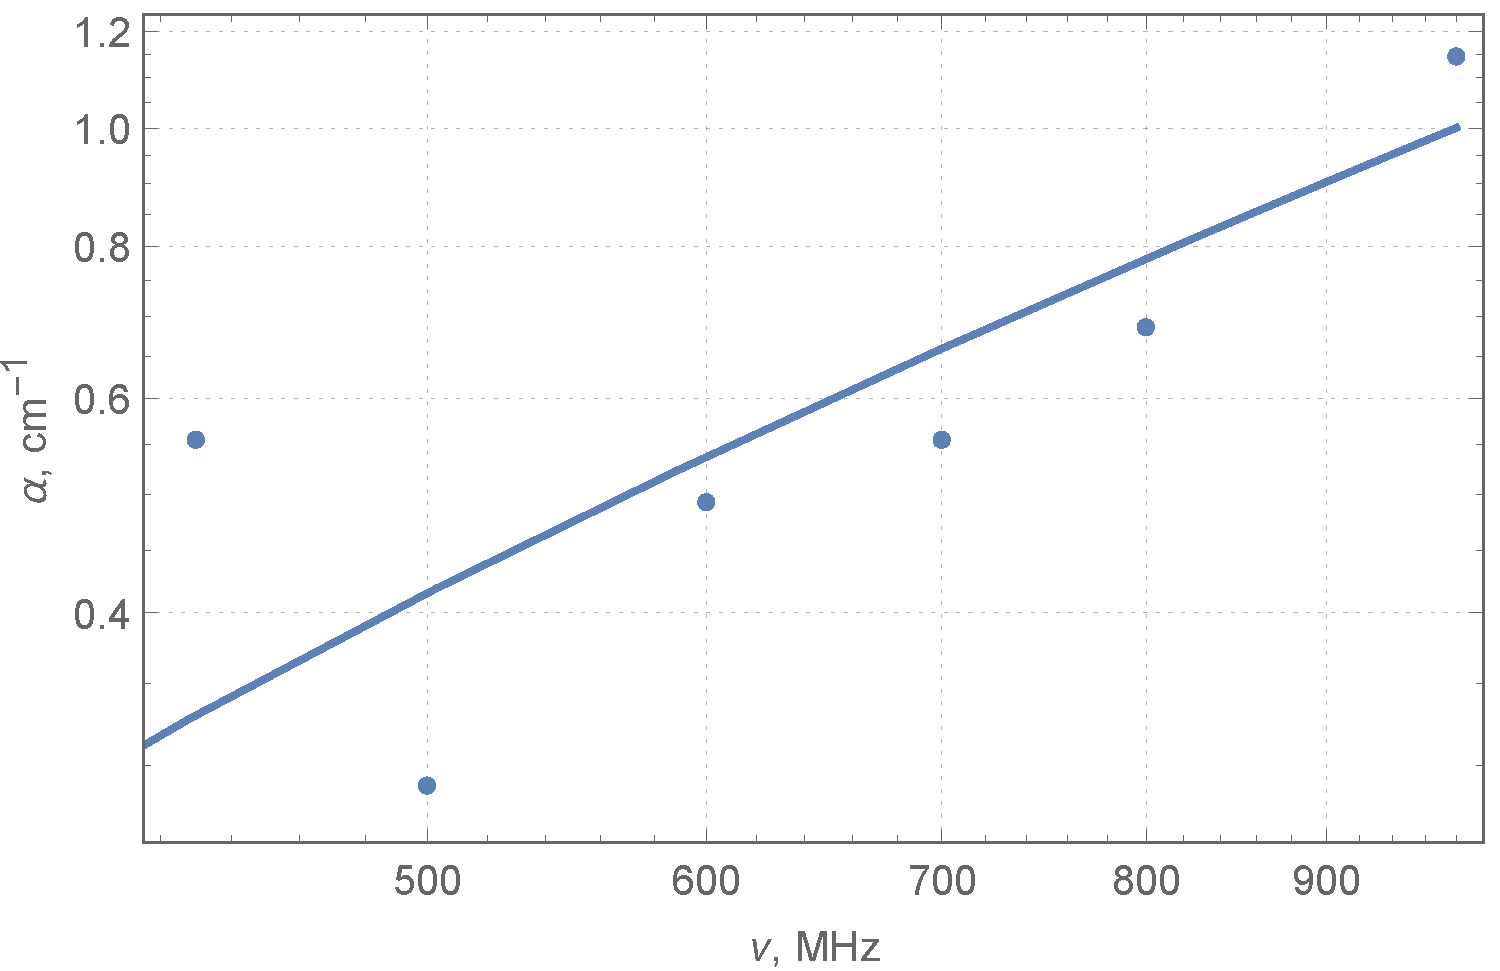
\includegraphics[width=0.7\linewidth]{graph}
    \caption{Зависимость $\cfrac{f^2}{f_0^2-f^2}(T)$}
\end{figure}

Линейный участок аппроксимируем прямой, искомые коэффициенты из метода наименьшних квадратов равны:

\[k = 8.86 \pm 0.40\]
\[b = -149.82 \pm 13.14\]

Пользуясь соотношениями \eqref{C-W} и \eqref{dependency}, получаем

\[\Theta = -\dfrac{b}{k} = 16.9 \pm 1.7~\text{$^\circ$C} = 289.9 \pm 1.7~\text{K}\]

Пользуясь формулой \eqref{obm-int}, оценим величину обменного интеграла, считая, что для гадолиния $n = 12$, $S = 7/2$:

\[J = 0.198\pm 0.019~\text{мэВ}\]

\section*{4. Выводы}
В ходе работы была исследована температурная зависимость магнитной восприимчивости гадолиния и определена температура Кюри $\Theta = 289.9 \pm 1.7~\text{К}$, что хорошо соответствует табличному значению $293.4~\text{К}$. По измеренным данным видно, что закон Кюри-Вейса не выполняется при температурах, ниже $\Theta$, т.е. в ферромагнитной области. По полученному значению $\Theta$ был оценен обменный интеграл $J = 0.198\pm 0.019~\text{мэВ}$.

\end{document}
